\documentclass[sigconf,nonacm,screen]{acmart}
\settopmatter{printfolios=true}
\geometry{a4paper}

%% PACKAGES %%
\usepackage[utf8]{inputenc}
\usepackage{microtype}
\usepackage[capitalise,nameinlink,noabbrev]{cleveref}
\usepackage{tikz}
\usepackage{subcaption}

\usepackage{natbib}

\usepackage[dvipsnames]{xcolor}
\usepackage[svgnames]{xcolor}


% random stuff for the coloured pearson corelation table
\usepackage[dvipsnames]{xcolor}
\usepackage[underline=true,rounded corners=false]{pgf-umlsd}

% \definecolor{pos-cor-very-weak}{HTML}  {FF0000}
% \definecolor{pos-cor-weak}{HTML}       {E3001C}
% \definecolor{pos-cor-moderate}{HTML}   {C60039}
% \definecolor{pos-cor-strong}{HTML}     {AA0055}
% \definecolor{pos-cor-very-strong}{HTML}{8E0071}
% \definecolor{neg-cor-very-weak}{HTML}  {71008E}
% \definecolor{neg-cor-weak}{HTML}       {5500AA}
% \definecolor{neg-cor-moderate}{HTML}   {3900C6}
% \definecolor{neg-cor-strong}{HTML}     {1C00E3}
% \definecolor{neg-cor-very-strong}{HTML}{0000FF}

\definecolor{pos-cor-very-weak}{HTML}  {FFFF00}
\definecolor{pos-cor-weak}{HTML}       {FFBF00}
\definecolor{pos-cor-moderate}{HTML}   {FF8000}
\definecolor{pos-cor-strong}{HTML}     {FF4000}
\definecolor{pos-cor-very-strong}{HTML}{FF0000}

\definecolor{neg-cor-very-weak}{HTML}  {00FFD0}
\definecolor{neg-cor-weak}{HTML}       {00BFDC}
\definecolor{neg-cor-moderate}{HTML}   {0080E8}
\definecolor{neg-cor-strong}{HTML}     {0040F3}
\definecolor{neg-cor-very-strong}{HTML}{0000FF}

\newcommand{\hcancel}[1]{%
    \tikz[baseline=(tocancel.base)]{
        \node[inner sep=0pt,outer sep=0pt] (tocancel) {#1};
        \draw[line width=0.5mm, black] (tocancel.south west) -- (tocancel.north east);
    }%
}%



% bring back the TODO command
\usepackage{soul}
\newcommand{\todo}[1]{ \large \sethlcolor{yellow} \hl{todo: |#1|}\PackageWarning{TODO:}{#1!} \normalsize }
\newcommand{\todoR}[1]{ \large \sethlcolor{red} \hl{todoR: |#1|}\PackageWarning{TODO:}{#1!} \normalsize }
\newcommand{\todoG}[1]{ \large \sethlcolor{green} \hl{todoG: |#1|}\PackageWarning{TODO:}{#1!} \normalsize }

\newcommand{\todoPi}[1]{ \large \sethlcolor{HotPink} \hl{todoPi: |#1|}\PackageWarning{TODO:}{#1!} \normalsize }

\newcommand{\todoB}[1]{ \large \sethlcolor{blue} \hl{todoB: |#1|}\PackageWarning{TODO:}{#1!} \normalsize }
\newcommand{\todoC}[1]{ \large \sethlcolor{cyan} \hl{todoC: |#1|}\PackageWarning{TODO:}{#1!} \normalsize }
\newcommand{\todoBB}[1]{ \large \sethlcolor{LightSkyBlue} \hl{todoBB: |#1|}\PackageWarning{TODO:}{#1!} \normalsize }
\newcommand{\todoBA}[1]{ \large \sethlcolor{Aquamarine} \hl{todoBA: |#1|}\PackageWarning{TODO:}{#1!} \normalsize }

\newcommand{\todoLg}[1]{ \large \sethlcolor{lightgray} \hl{todoLg: |#1|}\PackageWarning{TODO:}{#1!} \normalsize }


\newcommand{\todoP}[1]{ \large \sethlcolor{pink} \hl{todoP: |#1|}\PackageWarning{TODO:}{#1!} \normalsize }

\newcommand{\todoOl}[1]{ \large \sethlcolor{olive} \hl{todoOl: |#1|}\PackageWarning{TODO:}{#1!} \normalsize }
\newcommand{\todoBr}[1]{ \large \sethlcolor{Brown} \hl{todoBr: |#1|}\PackageWarning{TODO:}{#1!} \normalsize }
\newcommand{\todoOr}[1]{ \large \sethlcolor{orange} \hl{todoOr: |#1|}\PackageWarning{TODO:}{#1!} \normalsize }
\newcommand{\todoLi}[1]{ \large \sethlcolor{lime} \hl{todoLi: |#1|}\PackageWarning{TODO:}{#1!} \normalsize }
\newcommand{\todoPl}[1]{ \large \sethlcolor{Plum} \hl{todoPl: |#1|}\PackageWarning{TODO:}{#1!} \normalsize }


\newcommand{\paniktodo}[1]{ \normalfont }

% make subsubsection act like a regular section
\usepackage{titlesec}
\titleformat{\subsubsection}{\normalfont\Large\bfseries}{\thesubsubsection}{1em}{}

% exile over/underfull hbox warnings
\hbadness=99999
\vbadness=99999
\hfuzz=9999pt

% % % % % % % % % % % % % % % % % % % % %
%          STUDENT INFORMATION 
% % % % % % % % % % % % % % % % % % % % %
% \title{Relating Constraint Programming Techniques to Minesweeper Difficulty}
\title{Empirically Investigating Minesweeper Field Difficulty with Constraint Programming Techniques}

\author{Andrei Boghean} %% ENTER YOUR NAME HERE!!!
\affiliation{
  \country{2645295b} %% ENTER YOUR MATRICULATION NUMBER HERE!!!
}


%% DOCUMENT %%

\begin{document}
% % % % % % % % % % % % % % % % % % % % %
% 			ABSTRACT
% % % % % % % % % % % % % % % % % % % % %

\pagenumbering{roman}

\tableofcontents \hfill \\
\
repurposed (and commented unused highlights): \\
\todoB{BLUE} : \\explaining a paper, hence background \\
% \todoC{CYAN} : \\stuff to back up with research you've not found \\
\todoBB{SkyBlue} : \\expanding on a paper for some reason \\
\todoBA{Aquamarine} : \\creating design from a paper, hence design section \\
\todoOr{ORANGE} : \\explaining a compromise in the model, hence implementation? \\
% \todoLi{LIME} : \\logical curiosities to be refined \\
% \todoBr{BROWN}: \\ old stuff to be probably deleted \\

\hfill \\
% \todoB{BLUE} : \\stuff to genuinely research because you dont know \\
% \todoC{CYAN} : \\stuff to back up with research you've not found \\
% \todoBB{SkyBlue} : \\stuff to back up with research you've found but not inserted \\
% \todoBA{Aquamarine} : \\stuff you've backed up with research, but not finished reading the paper for \\
\todoR{RED} : \\logical curiosities to be figured out \\
% \todoOr{ORANGE} : \\logical curiosities to be written \\
% \todoLi{LIME} : \\logical curiosities to be refined \\
% \todoBr{BROWN}: \\ old stuff to be probably deleted \\
\todoPi{PINK}: \\ structural notes \\
\todoPl{PLUM}: \\ structural conclusions to be acted on \\
\todoLg{LIGHTGRAY}: \\ stuff broadly marked as "new" \\
\
pearson correlations colours: \\
\textcolor{pos-cor-very-weak}  {pos-cor-very-weak}
\textcolor{pos-cor-weak}       {pos-cor-weak}
\textcolor{pos-cor-moderate}   {pos-cor-moderate}
\textcolor{pos-cor-strong}     {pos-cor-strong}
\textcolor{pos-cor-very-strong}{pos-cor-very-strong} \\
\textcolor{neg-cor-very-weak}  {neg-cor-very-weak}
\textcolor{neg-cor-weak}       {neg-cor-weak}
\textcolor{neg-cor-moderate}   {neg-cor-moderate}
\textcolor{neg-cor-strong}     {neg-cor-strong}
\textcolor{neg-cor-very-strong}{neg-cor-very-strong}
\
first "draft" feedback notes: not sure what point \#12 says

% original layout:
%  0 \ref{awa:background} \nameref{awa:background} \\
%  1 \ref{awa:minesweeperGameContext} \nameref{awa:minesweeperGameContext} \\
%  2 \ref{awa:minesweeperImprovementDrive} \nameref{awa:minesweeperImprovementDrive} \\
%  3 \ref{awa:minesweeper3BVbad} \nameref{awa:minesweeper3BVbad} \\
%  4 \ref{awa:minesweeperNPcomplete} \nameref{awa:minesweeperNPcomplete} \\
%  5 \ref{awa:InferenceConsistencyRelation} \nameref{awa:InferenceConsistencyRelation} \\
%  6 \ref{awa:difficultyManipulationAttempts} \nameref{awa:difficultyManipulationAttempts} \\
%  7 \ref{awa:playerStudiedTechniquesAreProbabllyMostOfThem} \nameref{awa:playerStudiedTechniquesAreProbabllyMostOfThem} \\
%  8 \ref{awa:basicHHuristicsIntoAlgorithms} \nameref{awa:basicHHuristicsIntoAlgorithms} \\
%  9 \ref{awa:minimisingSudokuValue} \nameref{awa:minimisingSudokuValue} \\
% 10 \ref{awa:fieldQuantisingWithHeuristics} \nameref{awa:fieldQuantisingWithHeuristics} \\
% 11 \ref{awa:racIdentifiesTechniques} \nameref{awa:racIdentifiesTechniques} \\
% 12 \ref{awa:relationalArcConsistencyDiscussionMAYBE} \nameref{awa:relationalArcConsistencyDiscussionMAYBE} \\
% \\
% 13 \ref{sec:design} \nameref{sec:design} \\
% 14 \ref{awa:challengeSkillBallenceMonolith} \nameref{awa:challengeSkillBallenceMonolith} \\
% 15 \ref{awa:theHumanPlayingPipeline} \nameref{awa:theHumanPlayingPipeline} \\
% 16 \ref{awa:pathfindingWRTgameLogicStructure} \nameref{awa:pathfindingWRTgameLogicStructure} \\
% 17 \ref{awa:pathfindingCompromiseWithHumans} \nameref{awa:pathfindingCompromiseWithHumans} \\

\section{Background V2}
 0 \ref{awa:background} \nameref{awa:background} \\
 
    \subsection{The Current State of Minesweeper}
        \subsubsection{The Game of Minesweeper}
             1 \ref{awa:minesweeperGameContext} \nameref{awa:minesweeperGameContext} \\
        \subsubsection{Self-Improvement in Minesweeper}
             2 \ref{awa:minesweeperImprovementDrive} \nameref{awa:minesweeperImprovementDrive} \\
        \subsubsection{Improvement Indicators and their Usefulness}
             3 \ref{awa:minesweeper3BVbad} \nameref{awa:minesweeper3BVbad} \\
             
    \subsection{Minesweeper's Hardness}
         4 \ref{awa:minesweeperNPcomplete} \nameref{awa:minesweeperNPcomplete} \\
        \subsubsection{Kaye's Classification of Minesweeper Hardness}
        \subsubsection{Scott's Classification of Minesweeper Hardness}
        \subsubsection{Aside: Connection Between Perspectives}
             5 \ref{awa:InferenceConsistencyRelation} \nameref{awa:InferenceConsistencyRelation} \\

    \subsection{research into heuristics}
        \subsubsection{reusing some heuristics via algorithms}
             8 \ref{awa:basicHHuristicsIntoAlgorithms} \nameref{awa:basicHHuristicsIntoAlgorithms} \\
        \subsubsection{manipulating possible heuristics}
             6 \ref{awa:difficultyManipulationAttempts} \nameref{awa:difficultyManipulationAttempts} \\
             7 \ref{awa:playerStudiedTechniquesAreProbabllyMostOfThem} \nameref{awa:playerStudiedTechniquesAreProbabllyMostOfThem} \\
        \subsubsection{RAC is an algorithm for finding all strategies}
            11 \ref{awa:racIdentifiesTechniques} \nameref{awa:racIdentifiesTechniques} \\
            12 \ref{awa:relationalArcConsistencyDiscussionMAYBE} \nameref{awa:relationalArcConsistencyDiscussionMAYBE} \\
        
    \subsection{field manipulation from these methods}
        \subsubsection{field filtering}
            filtering is possible:
             9 \ref{awa:minimisingSudokuValue} \nameref{awa:minimisingSudokuValue} \\
             filtering application on minesweeper:
            10 \ref{awa:fieldQuantisingWithHeuristics} \nameref{awa:fieldQuantisingWithHeuristics} \\

\section{design V2}
13 \ref{sec:design} \nameref{sec:design} \\

    \subsection{the overarching model is logic, skill, pathfinding}
        \subsubsection{logic}
            logic is dictated by...
            logic can be dealt with by heuristics, and CP algs

        \subsubsection{skill}
            skill very simply begins with the player's grasp of all heuristics

        \subsubsection{pathfinding}
            pathfinding boils down to when the player decides they need to go somewehere else,
            and where they decide to go to.

            these 2 concepts break down further..
                when to leave? is there no value, can I not solve this, is it not fast enough, etc.
                where to go to? I remember this place seemed easy, or can try this unexplored place, or can guess
                    $\uparrow$ lots of luck in this portion

            14 \ref{awa:challengeSkillBallenceMonolith} \nameref{awa:challengeSkillBallenceMonolith} \\
            15 \ref{awa:theHumanPlayingPipeline} \nameref{awa:theHumanPlayingPipeline} \\
            16 \ref{awa:pathfindingWRTgameLogicStructure} \nameref{awa:pathfindingWRTgameLogicStructure} \\
            17 \ref{awa:pathfindingCompromiseWithHumans} \nameref{awa:pathfindingCompromiseWithHumans} \\

\section{implementation (going into experiment design?)}
    \subsubsection{logic implementation}
    \subsubsection{skill implementation}
    \subsubsection{pathfinding implementation}

\vfill
% \addtocounter{page}{-1}
\pagenumbering{arabic}
\setcounter{page}{0}
\todo{DELETE THIS CONTENT}

\begin{abstract}

Minesweeper is an NP-complete puzzle game whose random board generation can yield very different boards with drastically different solve difficulties, even within the same fixed board parameters, despite the simplicity of board generation.

Due to the unpredictability of this variance, there does not currently exist a difficulty metric that can capture it. Instead, players rely on metrics such as solve time and minimum clicks necessary, which are believed to be insufficiently representative.

This project studies factors contributing to the perceived field difficulty, including both player skill and field challenge,
to aid the creation of a more accurate difficulty metric for randomised minesweeper fields with fixed sizes and mine counts.

By looking at minesweeper as a constraint satisfaction problem, we can use well-established algorithms to objectively categorise the difficulty of different minesweeper moves, and subsequently apply this to both the moves needed to solve a board and the moves used by a player, in an effort to understand how the appearance of these different moves ultimately affects the time to solve the board.

The results of our experiment shows that CP techniques can directly estimate the solve time for a minesweeper playthrough from the computed logical complexity, but can not do so without processing the logical complexity from playthrough data, which defeats the purpose in its current state.
Our experiment also yields results that contradict the widely believed opinion that field difficulty isn't generally easily predictable, A conclusion which we believe isn't generalisable beyond our collected dataset due to insufficient data.

% 3BV has a strong positive correlation with solve time and logical difficulty, additionally having a strong negative correlation with the typical "reward" of a cell, correlations which contradict the widely believed opinion that 3BV is not representative of field difficulty.

Ultimately, we conclude that individual or even collected move difficulty is not the sole factor in a field's difficulty, but is a contributing factor that needs to be considered over many playthroughs, ideally every playthrough route possible on the field.
With this conclusion we also propose ideas for future work in enumerating all possible playthroughs of a field in a non-exhaustive but practically equivalent manner.

% Ultimately, we conclude that "harder" minesweeper fields are fields which place more importance on the path taken through a field by having path bottlenecks, where easier fields have no bottlenecks and can be solved by ignoring difficult sections until an alternative path is found.

% Our experiments are able to support some simple conclusions about player skill,
% and find that there is in fact a strong correlation between 3BV and time to solve, but can not definitively prove a correlation between 3BV and solve time across all possible minesweeper fields, since the experiment did not consider a broad enough selection of fields to allow this conclusion.
\todo{move some stuff to introduction}

% - as far as research into player skill goes, we did in fact make some surface level discoveries
% - as far as research into board analysis goes, we found that there's
%   a correlation between 3BV, field solve time, and field difficulty.
%   this is contradictory to what we would expect, as the author indicates 3BV is not in fact representative of difficulty.
%   reasons my experiment is flawed: only one 3bv score, small map size, small sample size, not trawling whole 3bv range.


% \todo{finish writing}
% Ultimately, we find that I dont have skill nor time to do this topic justice :(

% \todo{rewrite below}
% Minesweeper is NP-complete. as a fact of this, there are a variety of different algorithms that implement both non-exhaustive heuristics and full solutions for solving minesweeper. out of CP algorithms, relational arc consitency is the most practically applicable, and indeed this paper demonstrates RAC on a minesweeper field. from this paper, it can be seen that RAC with different parameters corespond to different moves of different difficulties.

% we can apply this to human playthroughs to learn what levels of difficulties different players are familar with \todoC{humans have an incomplete subset of perfect knowledge},
% and can then also apply this to minesweeper fields to learn what difficulties arise in the field. \todoBB{insert research about minesweeper clusters} \todoC{also some new research in this area?}

% combining this knowledge, we could subsequently reason about how well-equiped a human is with respect to a minesweeper field (see \todoC{elo}, something first poked at by \citet{whyArePuzzlesFun})
% however I dont have the data for that
\end{abstract}

%%%%%%%%%%%% DO NOT EDIT THIS PART!!! %%%%%%%%%%%%
%%%%%%%%%%%%%%%%%%%%%%%%%%%%%%%%%%%%%%%%%%%%%%%%%%
\maketitle
\tikz [remember picture, overlay] %
\node [shift={(0.5cm,-0.5cm)}] at (current page.north west) %
[anchor=north west,scale=0.7] %
{
\includegraphics{embeddables/CompSci_logo.pdf}};
%%%%%%%%%%%%%%%%%%%%%%%%%%%%%%%%%%%%%%%%%%%%%%%%%%
%%%%%%%%%%%%%%%%%%%%%%%%%%%%%%%%%%%%%%%%%%%%%%%%%%

% % % % % % % % % % % % % % % % % % % % %
% 			INTRODUCTION
% % % % % % % % % % % % % % % % % % % % %
\section{Introduction}
\label{sec:intro}
% This template is directly derived from ACM's
% \href{https://ctan.org/pkg/acmart?lang=en}{\texttt{acmart}} package; make sure
% to consult the corresponding
% \href{http://mirrors.ctan.org/macros/latex/contrib/acmart/acmart.pdf}{documentation}
% if you face any technical issues, or if you want to explore the full range of
% features offered.

% % % % % % % % % % % % % % % % % % % % %
% 	         BACKGROUND
% % % % % % % % % % % % % % % % % % % % %
\section{Background}
\label{awa:background}
% Perhaps you want to cite the seminal paper of \citet{Turing1937}, or
% prior~\cite{Goedel1931} and concurrent~\cite{Church1936} work.
\todo{SIGNPOSTING TEXT!!}

\subsection{The Game of Minesweeper} \label{awa:minesweeperGameContext}

Minesweeper is a popular logic game which was first released in 1989 as part of Microsoft Windows. It is a grid-based logic game, where the player is presented with a finite board featuring covered cells that may contain either a mine or an empty space. The player is tasked with uncovering all empty spaces on the board, usually done by deducing non-empty cells via the numbers inscribed on each cell stating the number of mines in the surrounding 8 cells.
In addition to the basic logic, the standard game also allows the player to keep track of mines by flagging suspected cells with mines, allows the player to execute a "chord" (explained bellow), and further helps them by automatically uncovering neighbours of a cell inscribed with 0. In the original game, the standard difficulties are comprised of Beginner (shown in \cref{fig:beginnerExample}), Intermediate, and Expert. These difficulties correspond to boards of 9 by 9 with 10 mines, 16 by 16 with 40 mines, and 30 by 16 with 99 mines (respectively).

\textit{chording} is a create-comfort feature which can be triggered on any revealed cell with a hint from one to eight, as long as the number of flags placed on the neighbouring cells (both immediate and diagonal) are equal to the hint number inscribed on the cell. The action itself will then open all neighbouring cells which are covered and un-flagged.

This feature is most used to save time and clicks when all cells are found in a 3x3 area, and is typically counted as the actual amount of mouse button clicks, meaning that there are less clicks actually counted compared to manually opening the neighbouring, known safe, cells.

\begin{figure}[htbp]
    \centering
    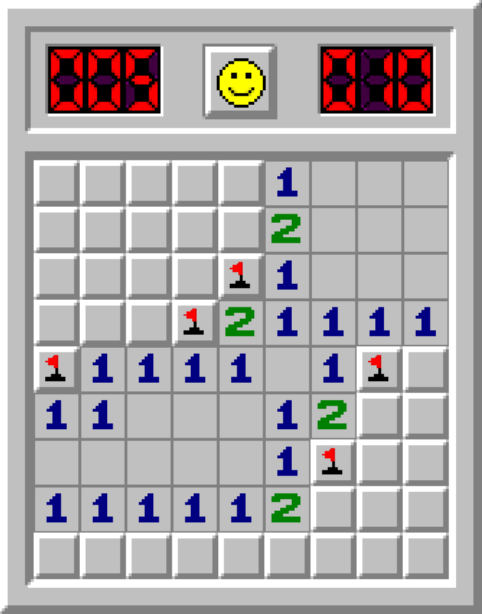
\includegraphics[width=0.5\linewidth]{embeddables/9x9ExampleBoardV2.png}
    \caption{A partially completed beginner board showing covered cells, covered cells flagged by the user, and opened cells with hints 0-8 indicating the number of neighbouring (both immediate and diagonal) mines.}
    \label{fig:beginnerExample}
\end{figure}

\subsection{Minesweeper Difficulty Metrics, their Purpose, and Flaws} \label{awa:minesweeperImprovementDrive}
% \subsubsection{Drive for improvement} \hfill \\
As with all games, particularly dedicated players aim to incrementally improve their skill, subject to some metric indicative of their performance. In minesweeper, there are two main metrics used in this process. The primary metric is solve time. For a player, solve time primarily serves as an objective reward which indicates how skilful the player was, and lets them adjust their methods accordingly over multiple plays to optimise their performance.

Solve time is not influenced just by player ability, but also by field difficulty.
When evaluating their play with the aim to improve, the player needs to "normalise" the performance they were expecting to display, to adjust for the field's difficulty.
\
This is why players typically try to improve over randomised placements of a fixed number of mines within a field of a fixed size, since it reduces difficulty variance, however games generated subject to these conditions still do not necessarily have the same difficulty over different randomisations, as different configurations can produce sequences of mines that might force more guesses, require moves of varying difficulty, bias speed of travel around the grid, capacity to memorise mines, pattern recognition, \textit{etc} (these ideas will be explained more concretely in \cref{sec:evaluation}).

In an effort to further mitigate this, \citet{3BVmetric} created the "3BV" score, a metric which simply counts the minimum number of necessary clicks to solve a board without using any flags. This is calculated upon completion of the board, and is used retrospectively by the player to adjust their belief on the quality of their performance.
% \todo{write an argument on scores being used retrospectively.}
\
This is still non-exhaustive, as is acknowledged by the creator of the aforementioned 3BV, who presents as an example two fields they had solved themselves in the same time (20s) with widely differing 3BV scores (38 and 72) shown below in \cref{fig:3BVbad}.
The general sentiment in the wider competitive Minesweeper community is similarly critical of its usefulness as a difficulty indicator on its own, as can be seen in some of the many online forum discussions on the topic\cite{redditComment1, redditComment2, redditComment3}.

\begin{figure}[htbp]
    \begin{subfigure}{0.22\textwidth}
        \centering
    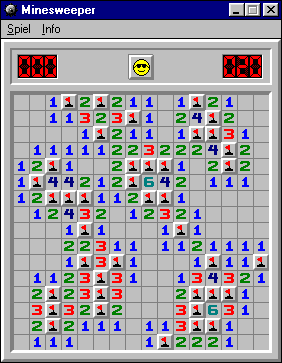
\includegraphics[width=0.9\textwidth]{embeddables/solved_20s_3bv38.png}
        \caption{20s field with a 3BV of 38}
        \label{fig:threebv38}
    \end{subfigure}
    \begin{subfigure}{0.22\textwidth}
        \centering
    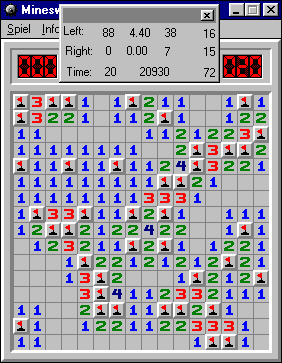
\includegraphics[width=0.9\textwidth]{embeddables/solved_20s_3bv72.png}
        \caption{20s field with a 3BV of 72}
        \label{fig:threebv72}
    \end{subfigure}
    \caption{Fields solvable in 20s with drastically different 3BV scores}
    \label{fig:3BVbad}
\end{figure}


\subsection{Problem Statement - need better than 3bv} \label{awa:minesweeper3BVbad}
So far there exists no metric or combination of metrics that can sufficiently capture the nuances in difficulty of minesweeper boards, and instead players must use a combination of surface-level metrics for a general estimation of difficulty instead.

Considering minesweeper's nature and its difficulty as an NP-hard game, as shown by \citet{kaye2000minesweeper} whose argument we'll explore below, we aim to explore the possibility for a CSP approach to provide a deeper insight into the difficulty of a minesweeper field and allow for more accurate estimation beyond the metrics explored, while also taking into account human factors and investigating how skill correlates to the expected "ideal" difficulty.



\subsection{Logical Complexity of Minesweeper - can use CP algs} \label{awa:minesweeperNPcomplete}
% framing of minesweeper: it's been called a "promise problem" \cite{minesweeperNPmeh}, it's been called a (partially observable) Markov decision problem \cite{msmarkovproblem}
The computational complexity of Minesweeper is well understood to be hard.
\
This fact was first established by a very popular paper by \citet{kaye2000minesweeper},
in which the author simplified minesweeper to what will be referred to as the "minesweeper consistency" problem.
\
This consistency problem is a sub-problem found in minesweeper, that is simpler than playing the whole game but still complex enough to capture the "core" difficulties of minesweeper's computational complexity.
\
\citet{kaye2000minesweeper} defines minesweeper consistency as a problem operating over "a rectangular grid, partially marked with numbers and/or mines, some squares being left blank" which asks whether there exists an assignment of mines to covered cells which is consistent with the numbers revealed in open cells (i.e. all cells numbered $x$ have exactly $x$ neighbouring mines).
\
To prove consistency is an NP-complete problem, \citet{kaye2000minesweeper} begins by establishing that minesweeper is in NP, by showing it is possible to transform a minesweeper field into a boolean satisfiability problem. He states this is done by isolating an arbitrary 3 by 3 grid of cells with a cleared middle cell stating n neighbouring mines, and argues this is equivalent to a boolean satisfiability problem where each clause is a different possible arrangement of mines among the neighbours, with the full 3 by 3 sub-grid being a disjunction of the possible $\begin{pmatrix}8 \\ n\end{pmatrix}$ hidden mine combinations. \citet{kaye2000minesweeper} then assembles these individual SAT problems for 3 by 3 sub-grids into a full statement for the whole board via conjunction.
\
To provide a polynomial time reduction from an NP-complete problem to minesweeper, \citet{kaye2000minesweeper} first shows that it is possible to create boolean logic circuits in minesweeper by showing how to create a simple wire via a mine arrangement where a designated output cell will contain a mine if and only if a designated input cell will contain a mine. \citet{kaye2000minesweeper} then extends this with wire bends and junctions, and finally boolean gates NOT and AND, which provides the basis for the other fundamental logic gates OR and XOR.
\
Using this digital computer, \citet{kaye2000minesweeper} shows how, for any instance of boolean satisfiability, a minesweeper circuit can be constructed where solving for consistency also solves the original SAT instance.
\
Having produced a proof for Minesweeper consistency being NP-complete, \citet{kaye2000minesweeper} then went on to generalise this sub-problem to the whole of Minesweeper, eventually concluding that a typical play through of the game is also NP-complete.

This conclusion is almost as widely accepted as their NP-completeness proof for Minesweeper consistency, but there is some disagreement.
\citet{minesweeperNPmeh} disputes \citet{kaye2000minesweeper}'s generalisation of NP-completeness from consistency to the game as a whole, on the basis that \citet{kaye2000minesweeper} did not consider the possibility that their proposed algorithm for solving general minesweeper via application of the consistency problem is not necessarily the most efficient method.
To explain their objection, \citet{minesweeperNPmeh} introduces a sister sub-problem to Minesweeper consistency - that of Minesweeper inference. This problem takes as input a board similar to consistency, with open cells, closed cells, and flags, and asks whether it is possible to make progress on the given board by identifying a cell as safe or containing a mine, subject to the condition that the board is already consistent and all flags are correct. Intuitively, this asks whether the only remaining actions on the field all force the player to guess, examples for which are shown in \cref{fig:inferenceExample}.
\citet{minesweeperNPmeh} demonstrates that the inference problem is in fact a co-NP problem, and subsequently presents a reduction from the unsatisfiability problem (the co-NP-complete variant of SAT) to Minesweeper inference through a very similar method to \citet{kaye2000minesweeper} - a general reduction for any (un)SAT problem to a computational circuit of logic gates, constructed through the rules of Minesweeper, that solves the respective problem when consistency is solved on the reduced minesweeper problem.

\begin{figure}[htbp]
    \begin{subfigure}{0.21\textwidth}
        \centering
        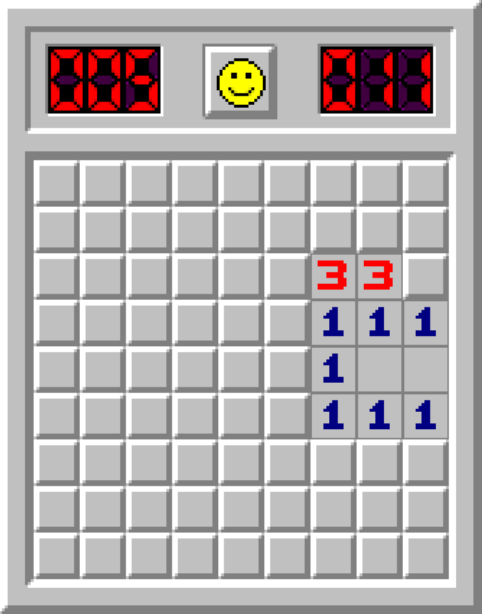
\includegraphics[width=\textwidth]{embeddables/progressableBoardV2.png}
        \caption{Field progressable\\without guessing}
        \label{fig:noGuess}
    \end{subfigure}
    \begin{subfigure}{0.21\textwidth}
        \centering
        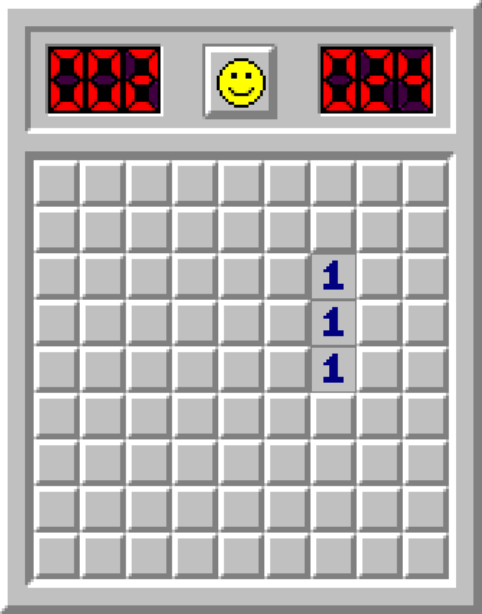
\includegraphics[width=\textwidth]{embeddables/unprogressableBoardV2.png}
        \caption{Field progressable only with guessing}
        \label{fig:guessOnly}
    \end{subfigure}
    \caption{partially solved fields that are progressable with and without guessing}
    \label{fig:inferenceExample}
\end{figure}

% \begin{figure}[htbp]
%     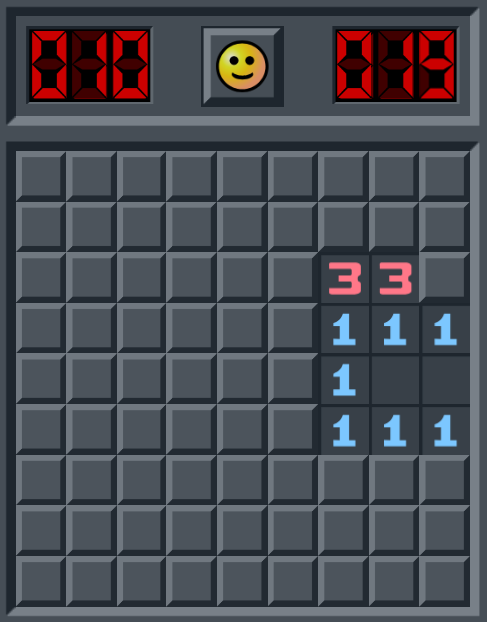
\includegraphics[width=0.20\textwidth]{embeddables/progressableBoard.png}
%     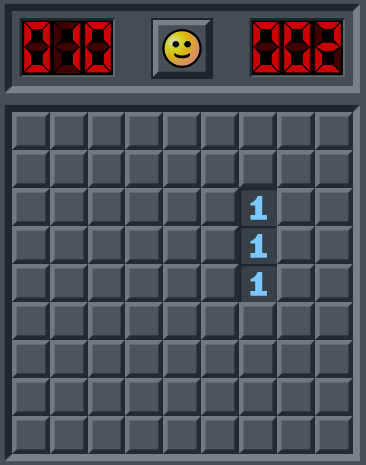
\includegraphics[width=0.20\textwidth]{embeddables/unprogressableBoard.png}
%     \caption{partially solved fields that are progress-able without guessing (left) and not (right)}
%     \label{fig:inferenceExample}
% \end{figure}

\subsubsection{Consistency/Inference Relation} \label{awa:InferenceConsistencyRelation}
\todoPi{this is an (I think) important extension to Inference and Consistency, but it's purely my own design, so I'm not sure I can put it in this section here and take it as fact?} \\
\todoPl{this will be explicitly stated as my own proposal/interpretation on a link between consistency/inference, and should likely be moved into the design somewhere}
\todo{re-write for better explanation}
\todoLg{In the context of a full minesweeper instance, these sub-problems do not suffice to make up the whole solving sequence. A full solve can be broken down into a repeated application of inference, where progress made on an individual instance of inference implicitly keeps the field "consistent".
\
Inference itself can also be defined in terms of consistency.
Inference can only be solvable when Consistency is solvable.
Inference on a field is possible when any cell on that field is solvable, without ambiguity.
This means that, in all possible solutions to Consistency, that same cell takes the same value all the time.
In the special case where there is only one solution to consistency, then Inference is possible on every cell, since no cell is ambiguous.
On the other hand, Inference on a field is not possible if every undecided cell has multiple possible options across all consistency solutions, i.e. there is always ambiguity.
\\
In other words, Inference asks whether the number of unambiguous cells across all Consistency solutions is greater than 0. If there are multiple unambiguous cells, then there are multiple Inference solutions.
\
While the computational complexity of a full minesweeper solve hasn't been explored, the individual steps still comprise NP-hard problems so our research into difficulty will need to focus on inference and develop methods to aggregate difficulty over the repeated occurrences that comprise the full solve of a minesweeper field.}
\\
% \todoOr{consistency but no inference means a forced guess.}
% \todoLi{ multiple consistency means multiple solutions. inference for a cell is only possible where all possible consistency solutions overlap for that cell.
% \\ \\
% no inference and multiple consistency means a forced guess \\
% one consistency solution means inference \\
% any inference and no consistency means there's been a mistake \\
% no inference and no consistency also means there's been a mistake }

% \todoPi{rewrite bellow til pink}
\subsection{Difficulty Manipulation via CSP Strategy Manipulation (MEH; rewrite, dont copy.)} \label{awa:difficultyManipulationAttempts}
\todoPi{this is begging to look into pathfinding, specifically manipulating the pathfinding options that arise whenever the player uses some heuristics or logic}
Knowing minesweeper can be classified as a constraint satisfaction problem, we can look to other studies investigating the difficulty of Constraint Satisfaction Puzzles, for insights that might extend to Minesweeper.
\
Specifically, we look at research in sourcing minesweeper heuristics, applying them, and lastly trying to manipulate them, in order to demonstrate the link between community-learned heuristics (patterns), and the perceived difficulty in the CSP game.

\subsubsection{sourcing common game strategies} \label{awa:playerStudiedTechniquesAreProbabllyMostOfThem}
\todoPi{player skill - says that a small subsection of techniques is already pretty sufficient} 
Before we can look at CSP strategies and how they relate to difficulty, we first need a way to identify strategies in the first place for investigation.
% \todo{place this somewhere with flow}
In \citeauthor{sudokuComputationalModel}'s research on encoding sudoku techniques into a computational model, they rely solely on techniques learned and documented by players through gameplay (specifically - techniques documented in popular puzzle solving books). While such a source may be non-exhaustive, it serves as a good starting point and likely includes most of the frequently encountered techniques.

% which may not seem academically sound, but other authors do the same suggesting community made materials are generally assumed safe by academia and appropriate to base findings on.

\subsubsection{research applying community-researched game strategies} \label{awa:basicHHuristicsIntoAlgorithms}
\todoPi{logical complexity - leading into heuristics that implement RAC}
In Minesweeper, there have been attempts to implement both classical (i.e. intuition or heuristics based) algorithms and constraint-based models, with some of these attempts basing themselves on previously identified human strategies and behaviours.

One such "classical" attempt is the "Single Point" strategy. the concept behind the single point strategy (SP) itself centres around the most common and simplest inferences or patterns that minesweeper players first learn, such as the one shown in \cref{fig:cornerexample}. The technique was formalised into the "single-point" strategy by \citeauthor{minesweeperSinglePoint}. Execution of SP starts by establishing an internal set of known valid moves, which the player picks moves from and executes. upon execution of a move, the set is refreshed with newly identified safe moves. Safe move identification is based on the simplest minesweeper technique - the identification of cases where the number in a cell is exactly equal to the number of neighbouring flagged cells which allows all neighbouring closed cells to be revealed, and secondly the identification of cases where the number of unopened neighbours is equal to the count of a cell, allowing the player to conclude that all neighbouring cells contain mines.

\citeauthor{minesweeperSolverShowdown} outlines a problem with the SP strategy where squares that did not immediately yield useful information are discarded prematurely. To mitigate this, they introduce a "Double Set Single Point" strategy. This strategy is defined as an extension to the simpler single point algorithm. Where SP would discard a square on a minesweeper field that does not fall into either of the 2 conditions for "progress", DSSP instead adds that square to a secondary set Q, that the algorithm returns to once it has exhausted all first-order squares with immediately accessible information for progress.

% \todo{argue the following: single point is just global arc consistency. DSSP is just global arc consistency, but with the memory to turn it into 2-RC, i.e. the next level in k-consistency.}

% \subsubsection{creating levels by manipulating "strategies"} \hfill \\
\subsubsection{research manipulating community-researched game strategies} \label{awa:minimisingSudokuValue}
\todoPi{remove? this is about storytelling in a linear game. minesweeper is non-linear with no story.}
\todoPi{besides the note on the line above, this section generally I think is pretty important in establishing pathfinding. I think it is the main chunk, taking a paper example and then explaining how it turns into the model. problem: it's a paper analysis intertwined with model definition. idk how to lead the fact that the paper reveals the concept of pathfinding, while not actually introducing it.}

In general game design, \citeauthor{marioEndless} focuses on combining mini levels together to form cohesive larger levels and create a "storyline" in a mario level. This is done by applying "Tension Arcs" which organises the order in which sub-levels are combined to maintain a smooth ramp-up in difficulty to a peak in the middle of the level which then starts to decay as the level finishes (effectively, the "story").

This notion of "difficulty regions" is also important in CSP games, for example in \citeauthor{sudokuGenerateBalancedHardness}'s research where they use the concept to get around scaling sudoku boards beyond sizes of 5 blocks (a block being a 3 by 3 sub-section), where the difficulty of solving increases drastically.

% This notion of "difficulty regions" is also present in other CSP games, for example \citeauthor{sudokuGenerateBalancedHardness} who addresses a challenge in generating sudoku boards where the "sub-block" construction of sudoku boards leads to significant jumps in difficulty as board block count increases, most notably at the boundary between 5 and 6 blocks.

To progress difficulty further while not having to scale the board size, they research board generation methods which "hide" complex combinations of constraints in generated fields to control the flow of difficulty.
\
Their approach starts with a given, complete, sudoku field, and creates permutations via specific permissible actions that rearrange the board in fashions which do not violate the rules.
\
They apply difficulty controls as rulesets for this generator,
with the core of their difficulty control being the "balance" of empty cells through rows, columns, and blocks.
\
Their difficulty balancing uses a network representation of sudoku boards, in which there is $n+m$ nodes for each $n$ rows and $m$ columns with nodes being connected if and only if that (row, column) position on the board contains an empty cell. Using this framing, they constrain their generator to enforce a regular bipartite graph, which effectively "balances" empty cells between rows and columns so there does not exist any disproportionately weighted node. Maintaining a node balance then ensures that empty squares are spread out and interact with each other minimally, so the user is only able to make slow consistent progress rather than solving a single empty square for a significant chunk of the board.

This balancing approach via a regular bipartite graph addresses the easiest method for progress in sudoku - filling out empty cells that are alone in an otherwise filled out row/column/block.
Sudoku, much like minesweeper and other logic games, has more complex techniques available to a player beyond the techniques mitigated by these surface-level balancing operations. While the demonstrated difficulty balancing only balances the usability of easier techniques, it brings up an important idea of "technique reward", whose average value and variance could impact the reward in a given map for luck or a gambling-focused play style.

\subsubsection{finding typical path difficulty, with heuristics, to categorise fields} \label{awa:fieldQuantisingWithHeuristics}
% \todoPi{this is kinda an attempt to simulate the skill factor, by using virtual agents with increasingly complex skill (instead of humans). this is also important for our future work in pathfinding, because we propose using this as a substitute for human playthroughs.}
\todoPi{this is broadly a pathfinding section. our future work would ultimately be full path enumeration, but this work is a stepping stone where it considers a small set of paths according to \textit{machines} of different skill. it's a further step than what I do, which is a small set of paths according to \textit{humans} of different skill} 
Getting closer to Minesweeper, \citet{minesweeperGeneration} creates a Minesweeper board generator, and much like \citet{sudokuComputationalModel} they also source field candidates via random placements. In their case however, presumably since Minesweeper boards are much more relaxed in their rules for "consistency", \citeauthor{minesweeperGeneration} does not need to use a complex board generator or permutation scheme. Instead, their approach constructs a board by randomly placing mines in an empty grid and using minesweeper solver algorithms to validate that inference is possible, proposing that this should guarantee the whole field is solvable.
% By the nature of \citeauthor{minesweeperGeneration}'s selected algorithms for inference checking, this generator might arrive at false negatives on some particularly complex generations, since the chosen solvers are not computationally perfect solvers and rather are primarily composed of good-enough polynomial solvers.
\citeauthor{minesweeperGeneration}'s chosen algorithms for inference validation starts with single point, secondly moves on to a backtracking algorithm with complex guessing, thirdly tries a "linear equation solver" which is self-described as an extension to single point, fourthly applies a good-enough polynomial time solver, and lastly tries an algorithm with exponential complexity. All of these algorithms, while increasingly complex, do not exhaustively solve all minesweeper instances and thus opens the generator to the possibility of false negatives on some particularly complex generations.
\todo{$\uparrow$ expand on the algorithms and why they're relevant}

This generator, with a wide selection of different solving options with increasing complexity, was found to be effective in selecting fields with specific "ranks" (the largest number of variables ever needed to consider in a single step in the whole field solve), ranging up to rank 9.

This validation method using increasingly complex solvers is effective at categorising fields according to worst-case difficulty, but doesn't reveal much difficulty information on individual moves beyond revealing the hardest move rank in a solve.





\subsection{Applicable Strategies Can Be Found by Relational Arc Consistency} \label{awa:racIdentifiesTechniques}
\todoPi{this section relates to both logic and skill. specifically, an implementation detail rather than any contribution to the model}
The approaches explored so far, which aim to understand and control difficulty,
demonstrate the important idea of "local difficulty" or "strategy biases" within their given problem.
That is, local portions of a problem instance that necessitate "harder" techniques to solve.

We might then want to look at similar strategy biases within minesweeper fields, to get a more granular understanding of how difficulty is affected.
A method for doing this is already partially demonstrated by \citet{minesweeperNConsistencyAssist}, who aims to create a tool, via constraint programming, to assist players in solving minesweeper fields.
To do this, they give the player the option to ask the computer to apply varying levels of the relational arc consistency algorithm, as defined by \citet{ConstraintProcessingBook}, for three different levels {1,2,3}-RC, and either solve all moves revealed by the algorithm or simply identify them.

Their use of Relational Arc Consistency inadvertently demonstrates how it can relate to minesweeper strategies of varying difficulty, as can be seen in \cref{fig:msRAC}. While their paper does not thoroughly study this relation, their demonstration still supports the idea and provides a good starting point in investigating how constraint satisfaction techniques relate to game solving heuristics learned by humans.

\begin{figure}[htbp]
    \centering
    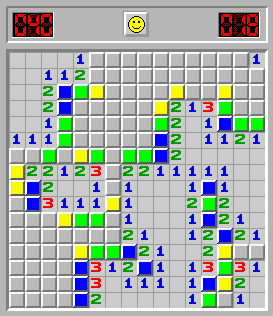
\includegraphics[width=0.5\linewidth]{embeddables/minesweeperTechniques.png}
    \caption{minesweeper field annotated with blue, green, and yellow illustrating possible progress discernable via 1, 2, and 3-RC respectively.}
    \label{fig:msRAC}
\end{figure}

\subsubsection{Relational Arc Consistency} \label{awa:relationalArcConsistencyDiscussionMAYBE}
\todo{insert rundown of RAC}

% % % % % % % % % % % % % % % % % % % % %
% 			YOUR SYSTEM
% % % % % % % % % % % % % % % % % % % % %
\section{Project "Design"}
\label{sec:design}
% small note for reference on the "design":
% we've established that minesweeper is NP-complete, that moves have individual difficulty and reward, and that RAC can be used to find move difficulty.
% We're interested in human-percieved difficulty, so instead of looking at playthroughs made by machines, we look at playthroughs made by players.
% we will prove that this is viable for recreating time to solve, and will state that future work should generate playthroughs in a human-like fashion to allow time prediction without humans actually playing. there is a lot of possible specialisation in this, e.g. by taking into account a human's learned techniques from past playthroughs.

As we've explored, the effective difficulty of a Minesweeper field as experienced by the player is very complex, with many contributing factors including actual logical complexity, player skill, and pathfinding (extende with luck as well) to name a few.
This section summarises the background and distils it into a over-arching model that tries to account for all the contributing factors explored so far that can affect the end-to-end difficulty when a human is solving a Minesweeper field.

\subsection{logical-complexity and player-skill balance} \label{awa:challengeSkillBallenceMonolith}
\todoPi{This section explains the tie between complexity and player skill, using paper evidence. This honestly belongs in the background I think, but it also concentrates the information into our model representation, which is part of our design. again a conflict where info should be separated, but I idk how to without removing the necessary context.}

% actual logical complexity has already been well-researched

\todoB{VVVVVVVVVVVVV}
As is covered across many articles of research such as those by \cite{skillChallengeBalance, skillChallengeBalanceAgain, SkillIssueTbh}, generally, logical complexity and player skill are two sides of the same coin which can be balanced to create the feeling of "flow".

\citet{skillChallengeBalanceAgain}outlines very specific conditions for flow state, which are generally met during Minesweeper gameplay,
but two conditions specifically are relevant for consideration here: 1. there is a balance between a user's perception of their skills and the offered challenge, and 2. the offered challenge is clear and unambiguous.


In Minesweeper (and most other CSP games), players are allowed to control the subject of their own attention and are fairly unconstrained.
Beyond the primary goal of field completion, players alter their behaviour in whatever way possible to optimise for solve time (the specific aim of "time" being primarily supported by \citet{skillChallengeBalance}).
\todoB{$\uparrow\uparrow\uparrow\uparrow\uparrow\uparrow\uparrow\uparrow\uparrow\uparrow\uparrow$}
\todoBA{VVVVVVVVVVVVVVV}
There are many ways a player could alter their behaviour such as their tendency to go for easy moves, their threshold for time sunk into a portion of a board before deviation, the tolerance for when to fall to a random guess, and ultimately their frustration level before ending the game and/or moving to a different field (to name a few).

Players adapt their behaviour in accordance with the aforementioned flow, which they optimise in an effort to achieve their best solve time.

The behavioural patterns mentioned above can be boiled down to the player asking themselves "where should I go" in response to "this place is not worth it".
We suggest that the logical complexity, player skill, and navigational factors relevant in this thought process is sufficient to explain the end-to-end difficulty experienced by a player.
However, because it is such a broad definition, this project cant reasonably test all such contributing factors in their entirety.
Instead, since the logical aspect is already very well-researched, we will focus on the human skill aspect and eventually suggest future work that could account for field exploration.
(\todo{note to self: this will be exhaustive enumeration of paths for non-determinism, and pattern-specific logging for a further improvement to the human aspect.})
\todoBA{$\uparrow\uparrow\uparrow\uparrow\uparrow\uparrow\uparrow\uparrow\uparrow\uparrow\uparrow$}

\todoOr{VVVVVVVVVVVVVVV}
Player skill is entirely defined by the player's abilities. We do not have any method to directly learn the player's abilities,
however we do have ways to directly measure a field's difficulty.
As a workaround, we can observe how players behave upon encountering mine arrangements of different difficulties, and use this instead as a test of skill.

For this purpose, we need a correct measure for the difficulty of a mine arrangement, and subsequently a collection of mine arrangements of varying difficulty.

While sourcing an exhaustive list of minesweeper techniques for use when analysing a Minesweeper playthrough would be helpful, such a list may be impossible to construct.
Minesweeper patterns are not restricted to simply the 8 neighbours of a cell. Patterns are formed from different neighbour combinations across multiple cells, and can span the whole board in some cases such as \ref{fig:longPattern}. Since patterns are so unconstrained, a collection of every pattern may boil down to a naive collection of every possible assignment of mines to a field.

Instead of trying to identify every different type of move made, we can use the aforementioned Relational Arc Consistency (RAC) algorithm, which can be repeatedly applied while progressively increasing parameters, to identify the number of constraints that had to be considered for the move to be possible. This groups moves according to their logical complexity, and lets us look at minesweeper moves in a purer form.
\todoOr{$\uparrow\uparrow\uparrow\uparrow\uparrow\uparrow\uparrow\uparrow\uparrow\uparrow\uparrow$}

% NOTE to self: this is, by definition, conjecture. it's 3 hours before teh deadline, so nothing can be done now, but you should fix it when you review this.
\subsection{Relating Humans Applying Minesweeper Techniques to Constraint Propagation (useful? pending rewrite)} \label{awa:theHumanPlayingPipeline}
\todo{distill maybe?}
\todoPi{this basically explains the human playing process, and relates it to pathfinding. it's kind-of more of what I said above, but thought-out from start to finish from a player's perspective}
% In the similar CSP problem of sudoku, \citet{sudokuComputationalModel} proposes that constraint propagation is not only more efficient than backtracking search, it is the natural approach humans take for constraint satisfaction problems. Their research does not directly address this claim, but it vaguely supports it and it is reasonable to expect this behaviour to appear in our findings as well.

\todoB{VVVVVVVVVVVVVVVVVVVVVV} \\
\todoPl{in this lil blue section, I'm basically explaining how RAC corresppnds to minesweeper techniques. I didnt realise that's what I was doing when I was writing it.. anyways: it should be moved to the paper that introduces the link between minesweeper techniques and RAC.}
As previously explored by \citet{sudokuComputationalModel}'s sudoku research, human CSP solving vaguely follows a particular protocol for how they apply their knowledge to play a game. Humans first start with the easiest techniques they are aware of, for example in minesweeper looking at "corner" cells (as illustrated in \cref{fig:cornerexample}) or any other cell where the number of hidden neighbours equals the number of indicated mines, i.e. techniques that only need one level of consistency to identify.

Second to this, when there are no more such instances the player can find within their area of focus, they fall to the next type of difficulty for the techniques they apply. In minesweeper, the next level of consistency includes patterns such as 1221 arrangements (shown in \cref{fig:1221example}) against a wall of closed cells, a case that tells the player there are 2 mines next to each other exactly parallel to the double 2s. Another such pattern is a 121 sequence against a wall, which indicates there is a single mine directly contacting each 1, and an empty cell contacting the 2. This pattern requires 2-consistency to identify because it is not identifiable from a single constraint stemming from a single open cell. In the 121 case, the presence of the 2 asserts there are 3 possible combination of mines: either both on the left, both on the right, or both at either end. The solver is not able to determine which of these cases are the correct arrangement, without noticing that the leftmost 1 rules out the possibilities of 2 mines being on the left, because that would mean 2 mines are present in the jurisdiction of a 1 which would not be consistent with 1 mine being in it's neighbourhood. the symmetric case on the other side with the other 1 eliminates the case where there are 2 cells on the rightmost side, leaving the only possibility /where there is 2 mines on either side of the 2's area. This pattern and others of similar complexity or harder are documented by \citet{msPatterns}.

\begin{figure}[htbp]
    \begin{subfigure}{0.21\textwidth}
        \centering
        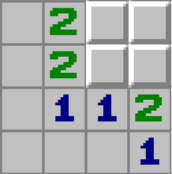
\includegraphics[height=2cm]{embeddables/easycornerSmallV2.png}
        \caption{Easy corner pattern}
        \label{fig:cornerexample}
    \end{subfigure}
    \begin{subfigure}{0.21\textwidth}
        \centering
        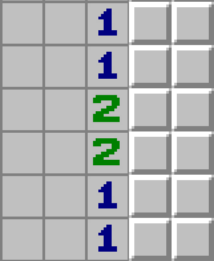
\includegraphics[height=2cm]{embeddables/1221smallV2.png}
        \caption{Slightly hard 1221 pattern}
        \label{fig:1221example}
    \end{subfigure}
    \caption{Minesweeper patterns of different difficulty}
    \label{fig:basicPatterns}
\end{figure}

After a human's known patterns are exhausted on a portion of the board, they may then fall back to their typical approach using constraint propagation to discern new patterns, where the player must enumerate possible states and progressively reduce them down to a reasonable solution. Alternatively, if the player has no known patterns whatsoever, they may also immediately go into this approach, a behaviour that's been observed by \citet{humanCSPapproach} on participants approaching unseen CSP challenges.
\todoB{$\uparrow\uparrow\uparrow\uparrow\uparrow\uparrow\uparrow\uparrow\uparrow\uparrow\uparrow$}

\subsection{human navigation of the minesweeper playing field} \label{awa:pathfindingWRTgameLogicStructure}
\todoPi{this is also pathfinding I think. Further, it's pathfinding in terms of the underlying structure of the complexity of the field (i.e. w.r.t. "clusters" as is defined by Cicvarek)}
what does it mean to be a "perfect" minesweeper player? \\
"imperfect" playing stems from the human nature to deviate on difficult portions of the board.. making "perfection" then means to remove the need to deviate, by augmenting the player/solver with the knowledge necessary.
\todoR{but what about the most basic path to take? even if you know every possible move, you still need to choose which of the possible moves to use, and where to go} \\

As a symptom of minesweeper's nature (\todoR{<-- what makes minesweeper a navigable game, and others not?}), playing a large enough game with an appropriate mine density can give rise to "clusters". These are defined, as by \citet{minesweeperGameGridGeneration}, to be groups of cells, where each constraint on each cell operates on other cells, who are also part of this cluster, i.e. there is no logical "connection" between clusters.

Thanks to this game structure, players can and do deviate from their current path very frequently as they approach moves they have not learned or cant apply easily.

In fact, \citet{whyArePuzzlesFun} (on a similar NP-complete puzzle game, Sokoban) considers this "deviation" to be fairly complex and highly varied from person to person or skillset to skillset, and worth researching. \todo{flesh out}

To understand the reasoning for this, we consider a typical minesweeper playthrough. A playthrough starts somewhere on the board with a random guess, and players continue randomly guessing until they strike a cell with a hint 0, which subsequently triggers the auto-reveal feature of Minesweeper \citet{minesweeperAutoreveal}.

Besides random guesses, there is in fact a more strategic guessing strategy. \citet{Studholme2001MinesweeperCSPencoding} suggests that, if the goal is to find a cell with a hint of 0, then it's most optimal to pick the cell with the least neighbours. The reasoning comes from the probability of a cell being empty, which is itself given by the probability of a single neighbour containing a mine, raised to the power of the number of neighbours. Since the probability of a neighbour containing a mine is between 0 and 1, the probability of the chosen cell having a neighbour with a mine can only decrease as neighbours increases.

Regardless of guessing strategy, the auto-revealed cells upon finding a 0-hint cell is then (usually) enough information for the player to start applying logical reasoning, learned heuristics, etc.

Among the newly revealed cells, the player can now either keep guessing to find more 0-hints (a technique used for an extra early boost in competitive play \todo{cite}) or start deciding on the next move according to the currently available information.

Deciding, then, can be informed by several strategies (these being listed in order of prerequisite experience needed):
the simplest but most inefficient strategy (beyond guessing) is simple brute-force.
assigning flags to various positions, and checking that their assignment holds within the wider context of the board (solving for consistency). \todo{citation for this}

second to this, possible moves can be identified by heuristics, patterns learned by the player from previous gameplay that can allow them to shortcut brute force enumeration and make a decision sooner.
\\
$\uparrow$ there is a great deal of nuance at this stage, depending on the player's experience. less experienced players with less learned patterns may identify less possible moves, and be more "starved" and hence gravitate strongly to the only moves they know.
Conversely, more experienced players with a more accessible playing field, have more choice in where they move.

This leads on to the next move decision strategy, "pathfinding".
Pathfinding refers to how the player navigates the aforementioned minesweeper clusters (something inexperienced players cant do, as they dont have the skill to "break in to" a cluster of difficult moves) and setting themselves up via move "entropy", the measure of how much information a given cell provides to the player upon making the move. On top of picking the closest move to minimise mechanical limits, advanced players may sacrifice a closer move for a further one, with more "entropy", because it gives more progress on the board overall.

\subsection{field pathfinding, or "luck"} \label{awa:pathfindingCompromiseWithHumans}
\todoPi{this section is about the navigational/pathfinding stuff mentioned in sec 3 "project design". specifically, how I sidestep it to allow the experiment to only focus on player skill without needing to consider pathfinding. it SHOULD NOT further refine the idea of pathfinding at all... the problem is that it does, because I've not refactored it. where should I move it? } \\
\todoPi{it also introduces "steppings stones" for pathfinding, explaining people-found paths as a compromise for full path enumeration}
\todo{actually, this section is unnecessarily verbose I think..} \\
% \todoLg{also this section} \\
\subsubsection{the design part}
we will outline the different ways people could deviate, 


\subsubsection{the implementation part}
to consider the typical difficulty for a minesweeper field, you of course need to consider the typical path.

theoretically, people arent necessary for this.
you may use a machine to enumerate every possible path,
and then draw conclusions on the field difficulty from that.

however, this is in practice of course very difficult because, for a 3bv value $x$ of (e.g. 40), there are $x$ different moves that all have to be made at one point or another. two different paths all have the same moves, just in a different order, hence there are $x!$ (e.g. $40! = 8.1591528 \cdot 10 ^{47}$) different possible field paths.

One may think that there is no practical need to enumerate every such path, and indeed that is correct.
consider the minesweeper pattern shown in \cref{fig:1221example}. The player can use logic to determine there are two discernible mines,
each being to the left of each of the twos shown. the player can subsequently deduce the square immediately north of the two mines is safe, and also that the square immediately south is safe.
The player can reveal the north square and then the south square, or the south square and then the north square.
alternatively, the player could only reveal the north square, and then proceed with the information they obtained from the north square, leaving the south square for later (this case also being mirrored).

Going for the north square is equivalent (within one move) to going for the south square, provided only that the player immediately goes for the south square afterwards.
Going for the north square and then proceeding elsewhere is NOT equivalent (within one move), and similarly going for the south square and proceeding elsewhere is also not equivalent.
This is given that we're considering equivalence over one move. all paths are eventually equivalent over the length of the playthough (provided it ends in a win)
\\ \\
The paths I've presented are only subtly different in the grand scheme of the playing field, and can be treated as practically equivalent as far as perceived difficulty is concerned.
\\ \\
Paths which are not perceptually equivalent, are paths which reveal different types of information earlier or later.
In the example, I glossed over picking the north cell and then deviating elsewhere (and the symmetric case) because I explain it now.
suppose the north cell contains a 1. In that case, the player is able to make deductions on the three west-most neighbours.
in such a case, the southern cell could be similarly easy, or be harder.

This gives rise to a complete guess, where the correct guess will lead to better performance, and the incorrect guess would not.

To make an effective difficulty metric, one would need to consider the average difficulty across all paths,
taking advantage of paths whose difficulty are practically equivalent and merging them in enumeration to cut down on the search space,
but still accounting for both paths in the computed average.
$\uparrow$ while still making sure not to merge different paths.

That may be done by checking practical equivalence within a distance of one move,
however this is just a heuristic and I suspect there's more to consider.

% % % % % % % % % % % % % % % % % % % % %
% 			EVALUATION
% % % % % % % % % % % % % % % % % % % % %
\section{Evaluation}
\label{sec:evaluation}
\todoLg{all of evaluation is of course also new.}

\subsection{Experimental Data}
    % \todoPi{EVALUATION IS BELOW..................}
    % \subsubsection{Sourcing a Dataset} \hfill \\
    \todo{jess suggestion: move some stuff to methods section?}
    In pursuit of a more representative difficulty metric for minesweeper fields, we must first source an objective ranking of fields, which can be cross-referenced for asserting correctness.
    
    When evaluating the field's challenge, simply the position of the mines is enough to estimate difficulty, however our aims necessitate data rich enough to recreate the individual moves made by the player in order to permit looking at how the player solves the discrete instances of the minesweeper Inference problem which comprise the full solve.
    
    Since there was no dataset fit for this purpose that was readily available, we collected playthroughs ourselves. This was achieved through a simple website, which presented the user with the typical experiment brief, debrief, instructions, and of course an implementation of the game itself.
    
    The implementation gave users one of the pre-selected maps (see \cref{table:pre-selected maps}), Tracked and recorded the type and timestamp of moves (cell reveals, flags, chords, restarts) and submitted them to a database together with anonymised user information, the map ID, and playthrough timestamp.
    
    % \subsubsection{Dataset Processing} \hfill \\
    To process the dataset, a RAC implementation similar to the one demonstrated by \citet{minesweeperNConsistencyAssist} was implemented to produce a final dataset where each move on each playthrough on each map is annotated with the corresponding "difficulty", given simply by the $m$ parameter necessary for RAC to deduce the move.
    
\subsection{Experimental Analysis}
    Our experimental analysis is split into 2 parts: field conclusions drawn from players, and player conclusions drawn from fields.
    Both field and player conclusions are viewed with respect to a ranking metric, where the metric is 3BV and player time advantage (as defined later in \ref{definePlayerSkill}) respectively.
    For these categories, we look at a selection of statistics which are chosen intentionally to ensure specific phenomena can be caught in analysis (if they indeed occur).
    
    \todo{eventually cut down the list of statistics.. right now they are more for personal reference thinking about what's worth including}
    \subsubsection{\textbf{statistics on Fields}} \hfill \\
        note: for every "statistic on a field" we could theoretically also compute them while filtering only to the solves of a specific person.
        this could be a step in the direction of "user-specific" map difficulty,
        however the problem is that I dont have the data to do this for every participant.
        also, even in an ideal system with every participant, this would only work on players which are dedicated. But, this may be fine since only the dedicated players would even be interested in this in the first place.

        \begin{enumerate}
            \item different maps having different randomly generated difficulties \\
            per-map distribution of move difficulties. \\
            also: for a specific map, a heatmap of the typical difficulty for each cell
        
            \item different maps having different minimum-skill requirements \\
            percentage completion
            
            \item different moves having different "payoffs" (with some moves being more useful to make than others) \\
            per-map move entropy heatmap
        
            \item \todo{number of moves to solve}
            
            \item \todo{number of moves to solve AS PERCENTAGE OF 3BV}
            
            \item "entry" points to solution. if there are multiple ways to solve, then the field is easy. if there is only one direction that leads to solving, then it's hard. \todo{write up why this is the end-goal, and why it's infeasible for me rn}
            
            \item \todo{heatmap of guesses}
        \end{enumerate}
    
    \subsubsection{\textbf{statistics on players}} \hfill \\
        \begin{enumerate}
            \item (experienced) players intentionally "skipping" easy moves for hard moves \\
            $\rightarrow$ player's percentage of moves (across all moves on any attempt on any field) where the player chose a further, harder, move when there was a nearby, easier, move available. (\todo{connect with cell entropy})
        
            \item (naive) players accidentally skipping hard moves because they're unaware \\
            $\rightarrow$ player's percentage of moves (across all moves on any attempt on any field) where the player chose a further, easier, move when there was a nearby, easier, move available. (\todo{connect with cell entropy})
            
            \item players playing faster or slower (according to skill) \\
            $rightarrow$ simply, a player's average time to make a move (across all moves on any attempt on any field).
            
            % \item (experienced) players placing a "hard" flag, so they can use a chord more efficiently \\
            % $\uparrow$ should be more common in low 3bv fields? high 3bv fields require many clicks by nature so there's less benefit to flagging. \\
            % $\rightarrow$ \todo{unimplemented}
        
            \item what action is taken when there's no lvl 1. moves available? \\
            $\rightarrow$ unimplemented and I dont understand what I was thinking
        
            \item more/less experienced players having more refined mechanics
            $\rightarrow$ average time spent per move difficulty. \\
        \end{enumerate}
    
    \subsubsection{\textbf{analysis methodology}} \hfill \\
        \todo{redo everything in evaluation :)} \\
        First, we need to test whether RAC actually corresponds to human minesweeping. \\
        we start with hypotheses stemming from anecdotal experience, and confirm/deny these using data. the more hypotheses get proven, the better RAC correlates?
        
        From review of submitted playthroughs and other ad-hoc playing, we identified a selection of phenomena that are either broadly important or demonstrate nuanced but interesting behaviour.
        Behaviour which, when viewed through a hypothetical "ideal" difficulty algorithm, should be discernible.
        
        These phenomena (in the form of hypotheses to be proven or disproven), together with their implementation as some statistic, are as follows:
        
        \begin{enumerate}
            \item \todo{"experienced" (i.e. difficulty actually encountered) difficulty through the solve}
            \item \todo{"experienced" (i.e. entropy actually used) entropy through the solve}
            
    \end{enumerate}
    
    \subsubsection{\textbf{analysis conclusion}} \hfill \\
        We can then look at some corresponding surface-level metrics which would be expected to reveal the corresponding phenomena.
        
        After applying these algorithms to the playthrough data, we can see the following trends: \\
        better people do indeed play faster \\
        ...
        correlations to look at:
        \begin{itemize}
            \item average times with 3bv
            \item 3bv with "difficulty"
            \item entropy with 3bv
        \end{itemize}
        
        oops ok I've looked at corelations, and I've found that 3bv is strongly corelated with time to solve
        which is contradictory.
        
        what is the problem? I only used one of each 3bv.
        why did I do this? because the original idea of this project wasnt focused on corelating solve time with 3bv, but instead solve time with 3bv across different player skills.
    
    \subsubsection{\textbf{defining player skill}} \label{definePlayerSkill} \hfill \\
        In investigating how player characteristics vary with player skill, we must first define what player skill is.
        This is difficult to define since not all players are playing with the same objective. Some players aim merely to complete the field, some players are aiming for speed, or some might be aiming to work on their technique rather than speed or even completion.
        By proportion, however, most players are aiming for solve time so our skill metric will be tailored as such.
        For a given player, we look at their percentage improvement with respect to the average time for a given field, and average this across all fields. This aims to factor out different fields that take different times to solve by their nature (\textit{e.g.} because they only take 2 clicks to solve).
    
    \subsubsection{Actual Experimental Results}
        In Minesweeper field evaluation, the 3 core metrics we decided to look at (average solve time, summed RAC difficulty, summed typical cell reward) are listed below in \ref{tab:fieldCoreStatistics}.
        Further below in \ref{tab:fieldCoreStatisticsPearson} is listed the Pearson correlation matrix between these variables.
        
        Our values claim 3BV has a moderately strong positive correlation with solve time, a very strong positive correlation with summed RAC difficulty, and a strong negative correlation with summed cell value.
        \todo{mention the p-values being < 0.05}
        The correlation between solve time and difficulty is as-expected and logical. The correlation between 3BV and difficulty/solveTime is initially surprising considering the doubt held by the Minesweeper community \todo{get a citation} on the correctness of 3BV, but our observation here is not generalisable to all minesweeper fields, since we have only considered one field for each of the 3BV scores selected for study.
        
        While this experiment design may theoretically be able to find Minesweeper fields with the same solve time but drastically different 3BV scores, it does not observe any fields with the same 3BV but drastically different solve times.
        
        it's also unknown how many participants were past the beginner phase and actively aiming for solve time rather than simply solving,
        however the criticism of 3BV only comes from players aiming to improve their solve time with respect to a specific difficulty, hence this dataset may not have playthroughs from the relevant audience and may not be able to deny the presence of a correlation.
        
        
        
        \begin{table}
        \footnotesize
        \begin{tabular}{llll}
        \toprule
            field 3BV & avg. solve time & summed RAC difficulty & summed typical cell reward \\
        \midrule
            % 14 &  29.08490 &  25.682927 &  36.257209 \\
             2 &   1.11 &   5.09 &  65.52 \\
             5 &  10.43 &   9.94 &  50.13 \\
             7 &  17.13 &  13.65 &  56.09 \\
             8 &  18.12 &   9.60 &  59.69 \\
             9 &  19.75 &  10.74 &  54.16 \\
            10 &  24.25 &   9.77 &  52.78 \\
            11 &  25.06 &  19.00 &  44.11 \\
            12 &  26.10 &  19.33 &  37.50 \\
            13 &  15.16 &  18.33 &  36.09 \\
            14 &  29.08 &  25.68 &  36.26 \\
            15 &  30.15 &  15.21 &  48.60 \\
            16 &  31.03 &  11.87 &  56.06 \\
            17 &  41.70 &  22.77 &  38.27 \\
            18 &  34.90 &  14.60 &  46.47 \\
            19 &  32.94 &  21.30 &  35.51 \\
            20 &  50.32 &  18.44 &  31.97 \\
            22 &  56.78 &  21.59 &  39.48 \\
            26 &  41.02 &  35.83 &  32.43 \\
            30 &  27.81 &  31.00 &  29.83 \\
            35 &  46.15 &  35.50 &  25.94 \\
            40 &  52.32 &  38.18 &  30.09 \\
        \bottomrule
        \end{tabular}
        \caption{Measured core field statistics.}
        \label{tab:fieldCoreStatistics}
        \end{table}
        
        \begin{table}[ht]
        \begin{tabular}{ccccc}
            % timeSolve & \textcolor{cor-very-strong}{1.0} & \textcolor{cor-strong}{0.79} & \textcolor{cor-strong}{0.68} & \textcolor{cor-very-weak}{-0.69}\\ \hline 
            % & timeSolve & 3BV & difficulty & cellReward\\ \hline 
            % 3BV &  & \textcolor{cor-very-strong}{1.0} & \textcolor{cor-very-strong}{0.9} & \textcolor{cor-very-weak}{-0.8}\\ \hline 
            % difficulty &  &  & \textcolor{cor-very-strong}{1.0} & \textcolor{cor-very-weak}{-0.88}\\ \hline 
            % cellReward &  &  &  & \textcolor{cor-very-strong}{1.0}\\ \hline
        
            % & 3BV & timeSolve & difficulty & cellReward\\ \hline 
            % 3BV & \textcolor{cor-very-strong}{1.0} & \textcolor{cor-strong}{0.79} & \textcolor{cor-very-strong}{0.9} & \textcolor{cor-very-weak}{-0.8}\\ \hline 
            % timeSolve &  & \textcolor{cor-very-strong}{1.0} & \textcolor{cor-strong}{0.68} & \textcolor{cor-very-weak}{-0.69}\\ \hline 
            % difficulty &  &  & \textcolor{cor-very-strong}{1.0} & \textcolor{cor-very-weak}{-0.88}\\ \hline 
            % cellReward &  &  &  & \textcolor{cor-very-strong}{1.0}\\ \hline 
        
            & 3BV & timeSolve & difficulty & cellReward\\ \hline 
            3BV & \textcolor{pos-cor-very-strong}{1.0} & \textcolor{pos-cor-strong}{0.79} & \textcolor{pos-cor-very-strong}{0.9} & \textcolor{neg-cor-strong}{-0.8}\\ \hline 
            timeSolve &  & \textcolor{pos-cor-very-strong}{1.0} & \textcolor{pos-cor-strong}{0.68} & \textcolor{neg-cor-strong}{-0.69}\\ \hline 
            difficulty &  &  & \textcolor{pos-cor-very-strong}{1.0} & \textcolor{neg-cor-very-strong}{-0.88}\\ \hline 
            cellReward &  &  &  & \textcolor{pos-cor-very-strong}{1.0}\\ \hline 
        \end{tabular}
        \caption{Pearson correlations between core field statistics}
        \label{tab:fieldCoreStatisticsPearson}
        \end{table}
        
        % \hfill \\ \\ \\
        % Our results are summarized in~\cref{tab:table1}, and a visual representation of
        % our analysis can be seen in~\cref{fig:basicPatterns}.
        
        % %% Example of table
        % \begin{table}
        % \footnotesize
        % \begin{tabular}{lll}
        % \toprule
        %          & machine A                   & machine B                           \\
        % \midrule
        % CPU      & Intel Core i7-9700 CPU      & 2x Intel Xeon E5-2630 v3            \\
        % CPU Frequency& 3.00GHz                     & 2.40GHz                             \\
        % RAM      & 16GB DDR4                   & 128GB                               \\
        % OS       & Ubuntu 20.04 LTS            & Ubuntu 16.04 LTS                    \\
        % Compiler & GCC 9.3                     & GCC 7.3                             \\
        % libm     & v2.31                       & v2.23                               \\
        % libomp   & v4.5                        & v4.5                                \\
        % \bottomrule
        % \end{tabular}
        % \caption{This is the table caption.}
        % \label{tab:table1}
        % \end{table}

% % % % % % % % % % % % % % % % % % % % %
%    CONCLUSIONS and FUTURE WORK
% % % % % % % % % % % % % % % % % % % % %
\section{Conclusions (0.5 page)}
\label{sec:conclusions}
In conclusion, Minesweeper is cool.

\section{Future Work (0.5 page)}
\label{sec:future_work}
basically: do the project again, but bigger and more.
more minesweeper fields across a wider range of the 3bv spectrum \\
more minesweeper fields among the same 3bv value. \\

$RAC_{(i, m)}$ only separates minesweeper moves as far as the number of constraints $m$  and number of variables $i$ needed to consider for a pattern to be recognised (recall that Generalised Arc Consistency is given by $RAC_{(1,1)}$, whereas $RC_2$ and $RC_3$ use an unbounded i, effectively meaning only the number of constraints is relevant beyond GAC). Within the same number of constraints, e.g. $RAC_1$ therefore, different types of moves that use the same difficulty but are a different pattern are treated as the same by us.
Future work then should modify Relational Arc Consistency with a form of proof logging, to assert which kind of pattern was used to make a conclusion about a cell. this information can then be used to record what specific type of patterns a person knows and is able to use, and ultimately build a better understanding of their capability to play minesweeper.
\\ \\
use larger values for RAC. also, track guesses.
\\ \\
I build statistics on a minesweeper field, e.g. the typical difficulty for a cell,
by looking at many playthroughs and storing the difficulty of the cell as sampled by the players, at the moment they clicked the cell, during their playthroughs.
effectively, I'm using the player playthroughs as exploration of the board
instead of carrying out exploration myself
because I dont want to create an algorithm for exploring the board.

currently, I substitute trying every single possible way to solve the board and use player playthroughs instead.
I then build statistics from that.

% % % % % % % % % % % % % % % % % % % % %
% 			ACKNOWLEDGMENTS
% % % % % % % % % % % % % % % % % % % % %
\section*{Acknowledgments}
I would like to thank caffeine.

% % % % % % % % % % % % % % % % % % % % %
% 			BIBLIOGRAPHY
% % % % % % % % % % % % % % % % % % % % %
\bibliographystyle{ACM-Reference-Format}
\bibliography{refs}
\end{document}
